\documentclass[a4paper]{article} 

\usepackage{listings}
\usepackage{xcolor}
\definecolor{codegreen}{rgb}{0,0.6,0}
\definecolor{codegray}{rgb}{0.5,0.5,0.5}
\definecolor{codeorange}{rgb}{1,0.49,0}
\definecolor{backcolour}{rgb}{0.95,0.95,0.96}

\usepackage{pgfplots}
\pgfplotsset{width=\textwidth,compat=1.9}

\lstdefinestyle{mystyle}{
    backgroundcolor=\color{backcolour},   
    commentstyle=\color{codegray},
    keywordstyle=\color{codeorange},
    numberstyle=\tiny\color{codegray},
    stringstyle=\color{codegreen},
    basicstyle=\ttfamily\footnotesize,
    breakatwhitespace=false,         
    breaklines=true,                 
    captionpos=b,                    
    keepspaces=true,                 
    numbers=left,                    
    numbersep=5pt,                  
    showspaces=false,                
    showstringspaces=false,
    showtabs=false,                  
    tabsize=2,
    xleftmargin=10pt,
}

\lstset{style=mystyle}

\addtolength{\hoffset}{-2.25cm}
\addtolength{\textwidth}{4.5cm}
\addtolength{\voffset}{-3.25cm}
\addtolength{\textheight}{5cm}
\setlength{\parskip}{0pt}
\setlength{\parindent}{0in}

%----------------------------------------------------------------------------------------
%	PACKAGES AND OTHER DOCUMENT CONFIGURATIONS
%----------------------------------------------------------------------------------------

\usepackage{blindtext} % Package to generate dummy text
\usepackage{charter} % Use the Charter font
\usepackage[utf8]{inputenc} % Use UTF-8 encoding
\usepackage{microtype} % Slightly tweak font spacing for aesthetics
\usepackage[english]{babel} % Language hyphenation and typographical rules
\usepackage{amsthm, amsmath, amssymb} % Mathematical typesetting
\usepackage{float} % Improved interface for floating objects
\usepackage[final, colorlinks = true, 
            linkcolor = black, 
            citecolor = black]{hyperref} % For hyperlinks in the PDF
\usepackage{graphicx, multicol} % Enhanced support for graphics
\usepackage{xcolor} % Driver-independent color extensions
\usepackage{marvosym, wasysym} % More symbols
\usepackage{rotating} % Rotation tools
\usepackage{censor} % Facilities for controlling restricted text
\usepackage{listings, style/lstlisting} % Environment for non-formatted code, !uses style file!
\usepackage{pseudocode} % Environment for specifying algorithms in a natural way
\usepackage{style/avm} % Environment for f-structures, !uses style file!
\usepackage{booktabs} % Enhances quality of tables
\usepackage{tikz-qtree} % Easy tree drawing tool
\tikzset{every tree node/.style={align=center,anchor=north},
         level distance=2cm} % Configuration for q-trees
\usepackage{style/btree} % Configuration for b-trees and b+-trees, !uses style file!
\usepackage{csquotes} % Context sensitive quotation facilities
\usepackage[yyyymmdd]{datetime} % Uses YEAR-MONTH-DAY format for dates
\renewcommand{\dateseparator}{-} % Sets dateseparator to '-'
\usepackage{fancyhdr} % Headers and footers
\pagestyle{fancy} % All pages have headers and footers
\fancyhead{}\renewcommand{\headrulewidth}{0pt} % Blank out the default header
\fancyfoot[L]{} % Custom footer text
\fancyfoot[C]{} % Custom footer text
\fancyfoot[R]{\thepage} % Custom footer text
\newcommand{\note}[1]{\marginpar{\scriptsize \textcolor{red}{#1}}} % Enables comments in red on margin

%----------------------------------------------------------------------------------------

\begin{document}

%-------------------------------
%	TITLE SECTION
%-------------------------------

\fancyhead[C]{}
\hrule \medskip % Upper rule
\begin{minipage}{0.295\textwidth} 
    \begin{raggedright}
        \footnotesize
        Andrew Hayes \hfill\\   
        21321503 \hfill\\
        a.hayes18@nuigalway.ie 
    \end{raggedright}
\end{minipage}
\begin{minipage}{0.4\textwidth} 
    \begin{centering}
        \large 
        CT2109 Assignment 3\\ 
        \normalsize 
    \end{centering}
\end{minipage}
\begin{minipage}{0.295\textwidth} 
    \begin{raggedleft}
        \footnotesize
        \today \hfill\\
    \end{raggedleft}
\end{minipage}

\medskip\hrule 
\medskip
\begin{centering}
    Double-Base Palindromes \& Complexity Analysis\\ 
\end{centering}
\medskip\hrule 
\bigskip

\section{Problem Statement}
The overall purpose of this assignment is to perform some basic complexity analysis on four distinct algorithms, each of which aim to achieve the same result: determining whether a String is palindromic.
More specifically, each algorithm will be fed the binary \& decimal representations of each integer between $0_{10}$ and $1,000,000_{10}$, in String form.
Each algorithm will then determine whether the String is palindromic, returning either \verb|true| or \verb|false|. 
Each method will have three counter variables to record the number of palindromes found: one for the numbers whose decimal form is palindromic, one for the numbers whose binary form is palindromic, and one 
for the numbers which are palindromic in both decimal \& binary form.
\\\\
The number of primitive operations will be recorded using a separate global variable for each method. 
Additionally, the real time taken by each method (in milliseconds) will be recorded. 
These measurements will form the basis of the complexity analysis performed.
The number of primitive operations will be recorded for each method and plotted against the size of the problem (the number of values being checked for palindromicity, $n$).
This graph should reflect the ``order'' of the problem, i.e. it should match the big-O representation derived from a time-complexity analysis of the algorithm.
For example, an exponential curve on the graph would indicate that the algorithm is of $O(n^2)$ complexity, while a straight line through the origin would indicate that the algorithm is of $O(n)$ complexity.

\section{Analysis \& Design Notes}
The first thing that we'll want to do in this program is declare the variables that we'll use to record the data for each method being tested. 
We will have seven arrays of size four, with one index for each method being tested. 
These arrays will be:
\begin{itemize}
    \item   \verb|long[] operations| - To count the number of primitive operations for each method.
    \item   \verb|int[] decCount| - To count how many numbers that are palindromic in decimal form are found using each method.
    \item   \verb|int[] binCount| - To count how many numbers that are palindromic in binary form are found using each method.
    \item   \verb|int[] bothCount| - To count how many numbers that are palindromic in both decimal \& binary form are found using each method.
    \item   \verb|long[] startTime| - To record the start time (in Unix epoch form) of the testing of each of the four methods.
    \item   \verb|long[] totalTime| - To record the total time (in milliseconds) by the testing of each of the four methods.
    \item   \verb|StringBuilder[] data| - This will be be used to create a String of CSV data for each method, which will be output to a \verb|.csv| file at the end of testing.
            Doing this saves us from having to open, write to, \& close a \verb|.csv| file every time we want to record some data, which would be very inefficient.
\end{itemize}

The first thing that we'll do in the main method is initialise all the indices in the \verb|StringBuilder[] data| array to have the appropriate headings from each column, one column for the number of primitive operations 
and one for the size of the problem that used that number of primitive operations, i.e. \verb|"operations,size\n"|.
\\\\
We'll also want to generate a two-dimensional array of all the Strings that we'll be testing for palindromicity, with one dimension for decimal Strings and one dimension for binary Strings, both going up to 
$1,000,000_{10}$.
Generating this once in the beginning will save us from having to re-generate the same Strings four times, which would be very inefficient.
\\\\
Each method that we will be testing will have its own class that implements the interface \verb|PalindromeChecker|. 
This interface will contain a single method with the signature \verb|public boolean checkPalindrome(String str)|. 
The reason for doing this will be to follow OOP principles \& the DRY principle so that we don't have unnecessary repetition of code. 
This will allow us to have one generic loop through each of the numbers from $0_{10}$ to $1,000,000_{10}$ instead of four separate ones.
Each of the methods that we will be testing will be overridden implementations of \verb|checkPalindrome|. 
We will have four classes that implement \verb|PalindromeChecker|:
\begin{itemize}
    \item   \verb|ReverseVSOriginal| - This class will contain ``Method One'' outlined in the assignment specification, which checks if a String is palindromic by comparing the String to a reversed copy of itself, hence the name.
    \item   \verb|IVersusIMinusN| - This will contain ``Method Two'' outlined in the assignment specification, which checks if a String is palindromic by looping through each character in the String using an iterator 
            \verb|i| and comparing the character at index \verb|i| to the character at index \verb|n-i|, where \verb|n| is the last index in the String, i.e., comparing the first character to the last, the second character to the second-last, etc.
    \item   \verb|StackVSQueue| - This will contain ``Method Three'' outlined in the assignment specification, which checks if a String is palindromic using essentially the same technique as ``Method Two'' 
            but instead of simply iterating through the String, each character of the String will be put onto both a Stack \& a Queue, and then items will be removed from the Stack \& Queue and compared to each other. 
            The LIFO nature of the Stack and the FIFO nature of the Queue result in this comparison being first character versus last, second character versus second-last, and so on.
    \item   \verb|RecursiveReverse| - This will contain ``Method Four'' outlined in the assignment specification, which checks if a String is palindromic using essentially the same technique as ``Method One'' 
            but using recursion to reverse the String instead of iteration.
\end{itemize}

An array called \verb|PalindromeCheckers[]| will be initialised to contain an instance of each of these four classes.
This array will be iterated over (using iterator \verb|j|) to test each method, which prevents code repetition.
In said loop, firstly, the \verb|startTime[j]| will be recorded using \verb|System.getCurrentTimeMillis();|. 
Then, a loop will be entered that iterators over each number between $0_{10}$ to $1,000,000_{10}$. 
Both the decimal \& binary Strings at index \verb|i| of the \verb|strings[]| array will be passed to \verb|palindromeCheckers[j].checkPalindrome()| to be checked for palindromicity.
Then, \verb|decCount[j]|, \verb|binCount[j]|, \& \verb|bothCount[j]| will be iterated or will remain unchanged, as appropriate.
\\\\
The count of primitive operations for each method will be iterated as they are executed.
I won't count the \verb|return| statements at the end of methods or accessing a variable or array index as primitive operations, as these (especially the \verb|return| statements) are computationally 
insignificant, and certainly aren't on the same level as something like creating a new variable in memory.
Unfortunately, it's not really possible to say with accuracy what is \& isn't a ``primitive operation'' in a language so high-level \& abstract as Java, but I feel that this is a reasonable approximation. 
We want to record the count of primitive operations at regular intervals of 50,000 during the process, so we will append the operations count and the current \verb|i| to \verb|data[j]| if \verb|i| is 
divisible by 50,000.
\\\\
Once the loop using iterator \verb|i| has ended, the total time taken will be recorded by subtracting the current time from the start time.
The number of palindromes found in decimal, binary, and both decimal \& binary will be printed out to the screen, along with the total time taken \& the total number of primitive operations for that method.
Finally, the data for that method will be written to a \verb|.csv| file. 
This will be repeated for all four methods in the \verb|palindromeCheckers| array.

\section{Code}
\lstinputlisting[language=Java, breaklines=true, title={NewPalindrome.java}]{../code/NewPalindrome.java}
\lstinputlisting[language=Java, breaklines=true, title={PalindromeChecker.java}]{../code/PalindromeChecker.java}
\lstinputlisting[language=Java, breaklines=true, title={ReverseVSOriginal.java}]{../code/ReverseVSOriginal.java}
\lstinputlisting[language=Java, breaklines=true, title={IVersusIMinusN.java}]{../code/IVersusNMinusI.java}
\lstinputlisting[language=Java, breaklines=true, title={StackVSQueue.java}]{../code/StackVSQueue.java}
\lstinputlisting[language=Java, breaklines=true, title={RecursiveReverse.java}]{../code/RecursiveReverse.java}

\newpage
\section{Testing}
\begin{center}
    \begin{tikzpicture}
        \begin{axis}[
                title={Number of Primitive Operations per Method},
                xlabel={Size of Problem},
                ylabel={Number of Operations}
            ]
            \addplot table [x=size, y=operations, col sep=comma] {../code/method0.csv};
            \addplot table [x=size, y=operations, col sep=comma] {../code/method1.csv};
            \addplot table [x=size, y=operations, col sep=comma] {../code/method2.csv};
            \addplot table [x=size, y=operations, col sep=comma] {../code/method3.csv};
            \legend{Iterative Reverse vs Original,$i$ vs $n-i$,Stack vs Queue,Recursive Reverse vs Original}
        \end{axis}
    \end{tikzpicture}
\end{center}

\begin{figure}[h]
    \centering
    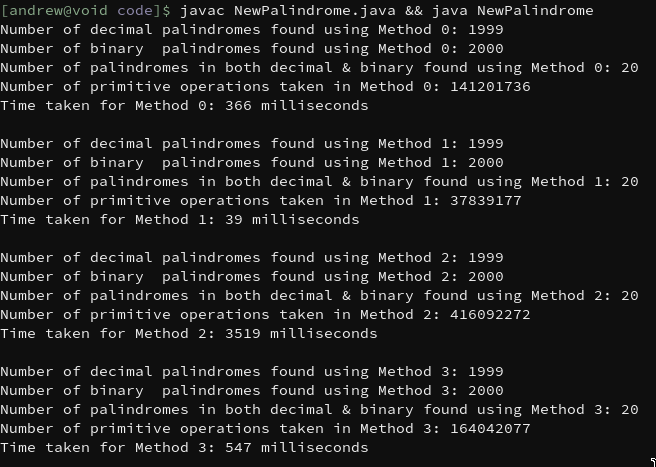
\includegraphics[width=0.7\textwidth]{images/output.png}
    \caption{Output of the Main Method}
\end{figure}

The output from the program shows that all the methods agreed on the number of palindromes found in each category, which shows us 
that they did indeed work as intended. 
\\\\
We can see from the graph that $i$ versus $n-i$ or \verb|IVersusNMinusI| method was the most efficient, as it used the fewest 
primitive operations out of the four methods (37,839,177) and the complexity grew relatively slowly as the size of the problem increased, 
demonstrated by the fact that its curve has quite a gentle slope.
This is reflected in the testing times as it was by far the fastest method (referred to in the screenshot as ``Method 1'', as 
indexing was done from 0), taking only 39 milliseconds to complete. 
This makes sense, as the method consisted of just one loop and some basic operations, without using any fancy data structures. 
Furthermore, this method quickly detects non-palindromic Strings, and returns \verb|false|, saving computation.
\\\\
The next most efficient method was the iterative reverse versus original or \verb|ReverseVSOriginal| method.
Despite being the next most efficient method, it took almost ten times the time that \verb|IVersusNMinusI| took to complete, taking 366 
milliseconds, which, all things considered, is still quite fast.
The number of primitive operations and the rate of growth of this method were also accordingly higher than the previous method.
\\\\
The third most efficient method was the recursive reverse versus original or \verb|RecursiveReverse| method. 
This makes sense, as it uses a very similar approach to the second most efficient method, but instead did it recursively. 
Despite this solution appearing somewhat more elegant from a lines of code perspective, it was in practice less efficient than 
its iterative counterpart, both in terms of memory (as the recursive function calls had to remain in memory until all the sub-calls 
were complete) and in terms of operations, taking approximately 20 million more primitive operations to complete the same task 
as the iterative approach.
It was also significantly slower than its iterative counterpart, taking around 200 milliseconds more to complete the task.
We can also tell from looking at the graph that at low problem sizes that this approach is comparable \& rather similar in terms 
of efficiency to the iterative approach, but they quickly diverge, with the recursive approach having a significantly steeper 
slope. 
We can extrapolate from this that this method would be even less efficient at very large problem sizes, as its rate of growth 
is quite large. 
\\\\
By far the least efficient method was the Stack versus Queue or \verb|StackVSQueue| method.
It took by far the greatest number of primitive operations, and the rate of growth was ridiculously large, rapidly diverging from 
the other four techniques.
Its rate of growth is so large that it would likely quickly become unusable for any significantly large problem. 
This is reinforced by the fact that it took 3,519 milliseconds to complete the task, being the only method that took more than one 
second to do so, and taking almost 100 times what the best-performing method took.

\end{document}
